\documentclass[letterpaper]{article} % Feel free to change this
\usepackage{graphicx}
\usepackage{caption}
\usepackage{rotating}
\usepackage{tabto}
\usepackage{amsmath}
\usepackage{listings}
\lstdefinestyle{mystyle}{
	basicstyle=\footnotesize,
	captionpos=b,
	numbers=left,
	showspaces=false,
	showtabs=false
}
\lstset{style=mystyle}
% comment out the next two lines if it doesn't compile for you
% or you could just install this package as well
\usepackage{vmargin}   
\setmarginsrb{1.0in}{1.0in}{1.0in}{1.0in}{12pt}{10mm}{12pt}{0mm}
\usepackage{fancyhdr}
 
\pagestyle{fancy}
\fancyhf{}
\rhead{ECE 538 Assignment 4}
\lhead{Alexander Zapata}
\rfoot{Page \thepage}
 
\begin{document}

\title{ECE 538: VLSI System Testing\\
\begin{large}{Assignment 4}\end{large}
\date{April 19, 2019}} % Change this to the date you are submitting
\author{Alexander Zapata}
\maketitle


\vspace{12.0cm}
\section*{Duke Community Standard}

By submitting this \LaTeX{} document, I affirm that
\begin{enumerate}
    \item I have adhered to the Duke Community Standard in completing this assignment.
\end{enumerate}

\newpage 

\section*{Problem 1 {\small Path	Delay	and	Small	Delay	Defect	Testing	using	Synopsys	TetraMax:}}
\subsection*{a. Path Delay Faults}
\subsubsection*{(i)}

\begin{table}[ht]
\centering
\begin{tabular}{|c|c|c|c|c|c|c|}
\hline
Number of Critical Paths & 50      & 100     & 150     & 200     & 250     & 300     \\ \hline
Total Faults             & 50      & 100     & 150     & 200     & 250     & 300     \\ \hline
Detected                 & 44      & 82      & 123     & 128     & 129     & 128     \\ \hline
Test Coverage            & 88.00\% & 82.00\% & 82.00\% & 64.00\% & 51.60\% & 42.67\% \\ \hline
Patterns                 & 9       & 18      & 19      & 19      & 19      & 18      \\ \hline
CPU Time                 & 0.02    & 0.02    & 0.03    & 0.02    & 0.03    & 0.05    \\ \hline
\end{tabular}
\caption{Results for path-delay faults, 0.15ns clock period}
\end{table}


\subsubsection*{(ii)}

\begin{table}[ht]
\centering
\begin{tabular}{|c|c|c|c|c|c|c|}
\hline
Number of Critical Paths & 50      & 100     & 150     & 200     & 250     & 300     \\ \hline
Total Faults             & 50      & 100     & 150     & 200     & 250     & 300     \\ \hline
Detected                 & 44      & 82      & 123     & 128     & 129     & 128     \\ \hline
Test Coverage            & 88.00\% & 82.00\% & 82.00\% & 64.00\% & 51.60\% & 42.67\% \\ \hline
Patterns                 & 9       & 18      & 19      & 18      & 19      & 18      \\ \hline
CPU Time                 & 0.01    & 0.03    & 0.03    & 0.03    & 0.03    & 0.04    \\ \hline
\end{tabular}
\caption{Results for path-delay faults, 0.10ns clock period}
\end{table}
The fault coverage for the 0.15ns/0.10ns path delay fault simulations were exactly the same. Having the same total faults, detected faults, and fault coverage means that--- from one timing to the next--- no additional delay faults were found on the critical paths tested (i.e., the paths not detected in the 0.15ns simulation had significant enough slack to also not be detected in the 0.10ns simulation). Between simulations, there was one more pattern for the 200 critical path simulation with 0.15ns clock than 0.10ns clock. This means that with the faster clock, fewer patterns were necessary to sensitize a delay long enough to detect. The CPU times were roughly the same for each simulation.

\subsection*{b. Small Delay Defects}
\subsubsection*{(i)}

\begin{table}[ht]
\centering
\begin{tabular}{|c|c|c|c|c|c|}
\hline
Slack               & 10\%            & 15\%             & 20\%            & 25\%             & 30\%            \\ \hline
Total Faults        & 4094            & 4094             & 4094            & 4094             & 4094            \\ \hline
Detected            & 3994            & 3994             & 3994            & 3994             & 3994            \\ \hline
Delay Effectiveness & 0.11ns(55.17\%) & 0.165ns(30.75\%) & 0.22ns(50.08\%) & 0.275ns(49.82\%) & 0.33ns(53.68\%) \\ \hline
SDQL                & 6289088.50      & 6126893.50       & 5438607.50      & 4897204.50       & 4477742.50      \\ \hline
CPU Time            & 0.07            & 0.07             & 0.07            & 0.08             & 0.08            \\ \hline
\end{tabular}
\caption{Results for small delay defects, 1.1ns clock period}
\end{table}


\newpage

\subsubsection*{(ii)}

\begin{table}[ht]
\centering
\begin{tabular}{|c|c|c|c|c|c|}
\hline
Slack               & 10\%           & 15\%            & 20\%            & 25\%            & 30\%            \\ \hline
Total Faults        & 4094           & 4094            & 4094            & 4094            & 4094            \\ \hline
Detected            & 3994           & 3994            & 3994            & 3994            & 3994            \\ \hline
Delay Effectiveness & 0.12ns(6.64\%) & 0.18ns(49.23\%) & 0.24ns(25.95\%) & 0.30ns(44.24\%) & 0.36ns(49.65\%) \\ \hline
SDQL                & 5756102.00     & 5206344.50      & 5301291.50      & 4501716.00      & 4122875.25      \\ \hline
CPU Time            & 0.08           & 0.06            & 0.07            & 0.07            & 0.08            \\ \hline
\end{tabular}
\caption{Results for small delay defects, 1.2ns clock period}
\end{table}
The delay-effectiveness for almost all simulations using 1.2ns clock period (with the sole exception of 15\% slack) was much lower than for the 1.1ns clock period simulations of the same slack-percentage. This means that fewer of the small delay defects could be detected in a circuit with a higher clock period. This is potentially because the small delay defects for a higher clock period (but with same percentage slack) have a longer path to sensitize--- so fewer tests will be able to do so. The SDQL values for the 1.1ns simulations are relatively higher than those for their 1.2ns simulation counterparts. This is most-likely the case because of the delay-defect distribution (i.e., there are more small-delay defects that with little slack when the clock period is relatively smaller). The CPU times stayed relatively the same.

\subsubsection*{(iii)}

\begin{table}[ht]
\centering
\begin{tabular}{|c|c|c|c|c|c|}
\hline
Slack               & 10\%            & 15\%            & 20\%            & 25\%            & 30\%            \\ \hline
Total Faults        & 4094            & 4094            & 4094            & 4094            & 4094            \\ \hline
Detected            & 3994            & 3994            & 3994            & 3994            & 3994            \\ \hline
Delay Effectiveness & 0.10ns(44.24\%) & 0.15ns(45.63\%) & 0.20ns(50.85\%) & 0.25ns(51.03\%) & 0.30ns(58.95\%) \\ \hline
SDQL                & 6445672.00      & 5683769.50      & 5567790.00      & 5023122.00      & 4668992.50      \\ \hline
CPU Time            & 0.07            & 0.08            & 0.08            & 0.08            & 0.08            \\ \hline
\end{tabular}
\caption{Results for small delay defects, 1.0ns clock period}
\end{table}
The delay-effectiveness is generally higher (with the exception of 10\% slack simulation) for the 1.0ns clock period simulations when compared to the 1.1ns clock period simulations. This most-likely means that there were shorter path lengths of the detected defects (within the slack-percentage), because the allowed slack was smaller. So, more shorter paths counted towards delay-effectiveness in the 1.0ns simulations. SDLQ fluctuated for the 1.1ns and 1.0ns simulations for which was higher for a given slack-percentage. Delay-effectiveness and SDQL was generally lower for the 1.2ns simulations compared to the 1.0ns simulations (presumably for similar reasons to the ones discussed in part ii).

\newpage

\section*{Problem 2 {\small Response compaction using LFSRs:}}
\subsection*{(c) Simulation Code and Results:}
\begin{lstlisting}[language=Python, caption=Python code used to simulate LFSR compaction]
	
#compact(flops, is_tapped, input_polynomial) simulates an LFSR given input params.
#flops- gives the instantiation value of the flip-flopsself.
#is_tapped- is asserted if the flop input should be tapped (Type-2 LFSR) high-order -> low-order.
#input_polynomial- the input bits that are xor'ed into the x^{n-1} flop in order.
def compact(flops, is_tapped, input_polynomial):
    into_one = False
    #Iterating through the input_polynomial bits.
    for i in range(len(input_polynomial)):
        #Setting temporary flops so that we can update sequentially.
        temp_flops = flops.copy()
        #Update each flop depending on tap value and value of previous flop.
        for j in range(len(flops)):
            if(is_tapped[j] == 1 and j != 0):
                temp_flops[j] = flops[len(flops) - 1] ^ flops[j - 1]
            else:
                if(j != 0):
                    temp_flops[j] = flops[j - 1]
        temp_flops[0] = input_polynomial[i] ^ flops[len(flops) - 1]
        #Set current values to updated values.
        flops = temp_flops
        #Printing result.
        print("Timestep Result " + str(i + 1) + ": " + str(flops))
    #Printing final flop values.
    for i in range(len(flops)):
        print("x^{}".format(i) + ": " + str(flops[i]))

#Calling the function with the values for the homework.
compact([0, 0, 0, 0], [1, 0, 0, 1], [1, 0, 1, 0, 1, 1, 1])
\end{lstlisting}

\begin{figure}[ht]
	\centering
	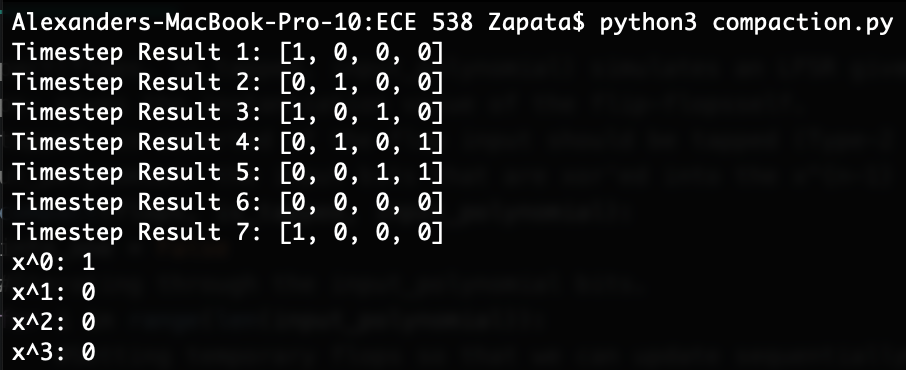
\includegraphics[width=10.0cm]{compaction_result.png}
\end{figure}
As can be seen in Figure 1, the result of the LFSR compaction was found to be a 1 in the $x^{0}$ register (i.e., a 1). This is the same result that was found by hand on the attached sheet.

\newpage

\section*{Problem 3 {\small SOC Test Infrastructure Design:}}
\hspace{0.5cm} To solve this problem, I used a heuristic BFD optimization algorithm (like discussed in class). The results and code are below.
\begin{table}[ht]
\centering
\begin{tabular}{|c|c|c|c|c|}
\hline
                                                                    & Wrapper SC 1                                                                                                    & Wrapper SC 2                                                                                                    & Wrapper SC 3                                                                                & Wrapper SC 4                                                                                                   \\ \hline
\begin{tabular}[c]{@{}c@{}}Wrapper\\ Internal SCs\end{tabular}      & \multicolumn{1}{l|}{\begin{tabular}[c]{@{}l@{}}Included:\\ - one 12-bit chain\\ - one 6-bit chain\end{tabular}} & \multicolumn{1}{l|}{\begin{tabular}[c]{@{}l@{}}Included:\\ - one 12-bit chain\\ - one 6-bit chain\end{tabular}} & \multicolumn{1}{l|}{\begin{tabular}[c]{@{}l@{}}Included:\\ - two 8-bit chains\end{tabular}} & \multicolumn{1}{l|}{\begin{tabular}[c]{@{}l@{}}Included:\\ - one 8-bit chain\\ - two 6-bit chain\end{tabular}} \\ \hline
\begin{tabular}[c]{@{}c@{}}Wrapper\\ Input Cells\end{tabular}       & 3                                                                                                               & 2                                                                                                               & 4                                                                                           & 0                                                                                                              \\ \hline
\begin{tabular}[c]{@{}c@{}}Wrapper\\ Output Cells\end{tabular}      & 2                                                                                                               & 3                                                                                                               & 3                                                                                           & 3                                                                                                              \\ \hline
\begin{tabular}[c]{@{}c@{}}Scan-in, Scan-out\\  Length\end{tabular} & 23                                                                                                              & 23                                                                                                              & 23                                                                                          & 23                                                                                                             \\ \hline
\end{tabular}
\caption{Wrapper design generated for embedded core C, TAM width of 4}
\end{table}

\begin{lstlisting}[language=Python, caption=Python code used to generate wrapper design.]
import math

def minimize_function(wrapper_chains, objects_to_add, activity_monitor, name):
    for i in range(len(objects_to_add)):
        min_chain = wrapper_chains.index(min(wrapper_chains))
        max_chain = wrapper_chains.index(max(wrapper_chains))
        minimum_chain_val = math.inf
        minimum_chain_num = -1
        for j in range(len(wrapper_chains)):
            value_to_minimize = wrapper_chains[max_chain] - (objects_to_add[i] + wrapper_chains[j])
            if((value_to_minimize >= 0) and (value_to_minimize < minimum_chain_val)):
                minimum_chain_val = value_to_minimize
                minimum_chain_num = j
        if(minimum_chain_num == -1):
            wrapper_chains[min_chain] += objects_to_add[i]
            activity_monitor[min_chain].append("{}: {}".format(name, objects_to_add[i]))
        else:
            wrapper_chains[minimum_chain_num] += objects_to_add[i]
            activity_monitor[minimum_chain_num].append("{}: {}".format(name, objects_to_add[i]))

def design_wrapper(tam_width, primary_input_num, primary_output_num, internal_scan):
    wrapper_chains = []
    activity_monitor = []
    for i in range(tam_width):
        wrapper_chains.append(0)
        activity_monitor.append(["Wrapper-Chain {}".format(i + 1)])
    #Step 1
    internal_scan.sort(reverse = True)
    minimize_function(wrapper_chains, internal_scan, activity_monitor, "sc")
    #Step 2
    primary_inputs = [1] * primary_input_num
    minimize_function(wrapper_chains, primary_inputs, activity_monitor, "pi")
    #Step 3
    primary_outputs = [1] * primary_output_num
    minimize_function(wrapper_chains, primary_outputs, activity_monitor, "po")
    activity_monitor.append("Final wrapper chains: {}".format(wrapper_chains))
    print(*activity_monitor, sep = "\n")
    return wrapper_chains

design_wrapper(4, 9, 11, [12, 12, 8, 8, 8, 6, 6, 6, 6])
\end{lstlisting}

\newpage

\section*{Problem 4 \small{SOC Testing:}}
\subsection*{(a)}
\hspace{0.5cm}The code used for problem 3 (in Listing 2) was used to design wrappers of the appropriate sizes\\ ($\text{w} = \text{2, 3, 4, 5, 6}$), the results are as tabulated below.
\begin{table}[ht]
\centering
\scalebox{0.75}{
\begin{tabular}{|c|c|c|}
\hline
                                                                    & Wrapper SC 1                                                                                                    & Wrapper SC 2                                                                                                    \\ \hline
\begin{tabular}[c]{@{}c@{}}Wrapper\\ Internal SCs\end{tabular}      & \multicolumn{1}{l|}{\begin{tabular}[c]{@{}l@{}}Included:\\ - one 12-bit chain\\ - one 8-bit chain\end{tabular}} & \multicolumn{1}{l|}{\begin{tabular}[c]{@{}l@{}}Included:\\ - one 12-bit chain\\ - one 8-bit chain\end{tabular}} \\ \hline
\begin{tabular}[c]{@{}c@{}}Wrapper\\ Input Cells\end{tabular}       & 8                                                                                                               & 8                                                                                                               \\ \hline
\begin{tabular}[c]{@{}c@{}}Wrapper\\ Output Cells\end{tabular}      & 4                                                                                                               & 4                                                                                                               \\ \hline
\begin{tabular}[c]{@{}c@{}}Scan-in, Scan-out\\  Length\end{tabular} & 32                                                                                                              & 32                                                                                                              \\ \hline
\end{tabular}
}
\caption{Wrapper design for width of 2}
\end{table}

\begin{table}[ht]
\centering
\scalebox{0.75}{
\begin{tabular}{|c|c|c|c|}
\hline
                                                                    & Wrapper SC 1                                                                                & Wrapper SC 2                                                                                & Wrapper SC 3                                                                               \\ \hline
\begin{tabular}[c]{@{}c@{}}Wrapper\\ Internal SCs\end{tabular}      & \multicolumn{1}{l|}{\begin{tabular}[c]{@{}l@{}}Included:\\ - one 12-bit chain\end{tabular}} & \multicolumn{1}{l|}{\begin{tabular}[c]{@{}l@{}}Included:\\ - one 12-bit chain\end{tabular}} & \multicolumn{1}{l|}{\begin{tabular}[c]{@{}l@{}}Included:\\ - two 8-bit chain\end{tabular}} \\ \hline
\begin{tabular}[c]{@{}c@{}}Wrapper\\ Input Cells\end{tabular}       & 7                                                                                           & 7                                                                                           & 2                                                                                          \\ \hline
\begin{tabular}[c]{@{}c@{}}Wrapper\\ Output Cells\end{tabular}      & 3                                                                                           & 2                                                                                           & 3                                                                                          \\ \hline
\begin{tabular}[c]{@{}c@{}}Scan-in, Scan-out\\  Length\end{tabular} & 22                                                                                          & 21                                                                                          & 21                                                                                         \\ \hline
\end{tabular}
}
\caption{Wrapper design for width of 3}
\end{table}

\begin{table}[ht]
\centering
\scalebox{0.75}{
\begin{tabular}{|c|c|c|c|c|}
\hline
                                                                    & Wrapper SC 1                                                                                & Wrapper SC 2                                                                                & Wrapper SC 3                                                                               & Wrapper SC 4                                                          \\ \hline
\begin{tabular}[c]{@{}c@{}}Wrapper\\ Internal SCs\end{tabular}      & \multicolumn{1}{l|}{\begin{tabular}[c]{@{}l@{}}Included:\\ - one 12-bit chain\end{tabular}} & \multicolumn{1}{l|}{\begin{tabular}[c]{@{}l@{}}Included:\\ - one 12-bit chain\end{tabular}} & \multicolumn{1}{l|}{\begin{tabular}[c]{@{}l@{}}Included:\\ - one 8-bit chain\end{tabular}} & \begin{tabular}[c]{@{}c@{}}Included:\\ - one 8-bit chain\end{tabular} \\ \hline
\begin{tabular}[c]{@{}c@{}}Wrapper\\ Input Cells\end{tabular}       & 2                                                                                           & 2                                                                                           & 6                                                                                          & 6                                                                     \\ \hline
\begin{tabular}[c]{@{}c@{}}Wrapper\\ Output Cells\end{tabular}      & 2                                                                                           & 2                                                                                           & 2                                                                                          & 2                                                                     \\ \hline
\begin{tabular}[c]{@{}c@{}}Scan-in, Scan-out\\  Length\end{tabular} & 16                                                                                          & 16                                                                                          & 16                                                                                         & 16                                                                    \\ \hline
\end{tabular}
}
\caption{Wrapper design for width of 4}
\end{table}

\newpage

\begin{table}[ht]
\centering
\scalebox{0.75}{
\begin{tabular}{|c|c|c|c|c|c|}
\hline
                                                                    & Wrapper SC 1                                                                                & Wrapper SC 2                                                                                & Wrapper SC 3                                                                               & Wrapper SC 4                                                          & \multicolumn{1}{l|}{Wrapper SC 5} \\ \hline
\begin{tabular}[c]{@{}c@{}}Wrapper\\ Internal SCs\end{tabular}      & \multicolumn{1}{l|}{\begin{tabular}[c]{@{}l@{}}Included:\\ - one 12-bit chain\end{tabular}} & \multicolumn{1}{l|}{\begin{tabular}[c]{@{}l@{}}Included:\\ - one 12-bit chain\end{tabular}} & \multicolumn{1}{l|}{\begin{tabular}[c]{@{}l@{}}Included:\\ - one 8-bit chain\end{tabular}} & \begin{tabular}[c]{@{}c@{}}Included:\\ - one 8-bit chain\end{tabular} & None                              \\ \hline
\begin{tabular}[c]{@{}c@{}}Wrapper\\ Input Cells\end{tabular}       & 0                                                                                           & 0                                                                                           & 4                                                                                          & 4                                                                     & 8                                 \\ \hline
\begin{tabular}[c]{@{}c@{}}Wrapper\\ Output Cells\end{tabular}      & 1                                                                                           & 1                                                                                           & 1                                                                                          & 1                                                                     & 4                                 \\ \hline
\begin{tabular}[c]{@{}c@{}}Scan-in, Scan-out\\  Length\end{tabular} & 13                                                                                          & 13                                                                                          & 13                                                                                         & 13                                                                    & 12                                \\ \hline
\end{tabular}
}
\caption{Wrapper design for width of 5}
\end{table}

\begin{table}[ht]
\centering
\scalebox{0.75}{
\begin{tabular}{|c|c|c|c|c|c|c|}
\hline
                                                                    & Wrapper SC 1                                                                                & Wrapper SC 2                                                                                & Wrapper SC 3                                                                               & Wrapper SC 4                                                          & \multicolumn{1}{l|}{Wrapper SC 5} & \multicolumn{1}{l|}{Wrapper SC 6} \\ \hline
\begin{tabular}[c]{@{}c@{}}Wrapper\\ Internal SCs\end{tabular}      & \multicolumn{1}{l|}{\begin{tabular}[c]{@{}l@{}}Included:\\ - one 12-bit chain\end{tabular}} & \multicolumn{1}{l|}{\begin{tabular}[c]{@{}l@{}}Included:\\ - one 12-bit chain\end{tabular}} & \multicolumn{1}{l|}{\begin{tabular}[c]{@{}l@{}}Included:\\ - one 8-bit chain\end{tabular}} & \begin{tabular}[c]{@{}c@{}}Included:\\ - one 8-bit chain\end{tabular} & None                              & None                              \\ \hline
\begin{tabular}[c]{@{}c@{}}Wrapper\\ Input Cells\end{tabular}       & 0                                                                                           & 0                                                                                           & 4                                                                                          & 4                                                                     & 8                                 & 0                                 \\ \hline
\begin{tabular}[c]{@{}c@{}}Wrapper\\ Output Cells\end{tabular}      & 0                                                                                           & 0                                                                                           & 0                                                                                          & 0                                                                     & 4                                 & 4                                 \\ \hline
\begin{tabular}[c]{@{}c@{}}Scan-in, Scan-out\\  Length\end{tabular} & 12                                                                                          & 12                                                                                          & 12                                                                                         & 12                                                                    & 12                                & 4                                 \\ \hline
\end{tabular}
}
\caption{Wrapper design for width of 6}
\end{table}

\subsection*{(b)}
\hspace{0.5cm}Knowing the acceptable widths of the wrappers, and the fact that each of the 8 SOCs are identical, greatly simplified this problem. The following code was used to maximize the minimum wrapper width for this TAM design (minimizing scan-in/scan-out length and therefore minimizing test-time).

\begin{lstlisting}[language=Python, caption=Python code used to minimize TAM test time for the given SOC design]
	
def tam_designer(total_width, wrapper_widths, num_cores):
    wrapper_widths.sort(reverse = True)
    tam_routes = [0] * num_cores
    for i in range(len(wrapper_widths)):
        if((sum(tam_routes) == 0) or (sum(tam_routes) > total_width)):
            for j in range(num_cores):
                tam_routes[j] = wrapper_widths[i]
    while(sum(tam_routes) < total_width):
        min_index = tam_routes.index(min(tam_routes))
        tam_routes[min_index] += 1
    return tam_routes

print(tam_designer(36, [2, 3, 4, 5, 6], 8))
\end{lstlisting}

In the TAM design result, each embedded core wrapper is given their own TAM lines; however, the TAM width is not the same for each core because of the 36-bit TAM width constraint. No wrappers share TAM lines in this case, as preempting tests would result in longer maximum test time for the given widths. Four of the wrappers will have a TAM width of 5 and the other will have TAM widths of 4. This ensures the maximum scan-in/scan-out time is 16 clock cycles, corresponding to the BFD optimization in part (a) and assuming one clock cycle per single-bit shift-in/shift-out.

\newpage

\section*{Problem 5 {\small Test Compression:}}
\subsection*{(a)}
\hspace{0.5cm}To generate the fan-out design for this problem, I used a heuristic method of determining a compressed width set of test inputs given a pseudo-random test-pattern set. To do this, I generated a conflict-graph (as discussed in class), from the compatibility and inverse compatibility of the test patterns for each scan chain, and then heuristically found a graph coloring that would lead to a sufficiently compacted input-line set. To find a relatively small graph-coloring, the order of the graph-coloring was randomly assigned and the coloring was computed n-times for n randomized node sequences. The computed coloring with minimum number of colors was then chosen. Note: an exhaustive search for the chromatic-number of the conflict graph was not done as algorithms to compute an exact result are $\mathcal{NP}$-complete and on the time-order of $O(2^{n}n)$. The code used to find the pseudo-random test patterns, conflict graph, graph-coloring, and the resulting fanout decompressor are below:

\begin{lstlisting}[language=Python, caption=Python code used to generate test-patterns; produce the conflict graph; and color the graph]
import random

def generate_patterns(num_chains, chain_lengths, num_patterns):
    pattern_holder = []
    vals = []
    random.seed(7)
    for i in range(95):
        vals.append('X')
    for i in range(3):
        vals.append('0')
    for i in range(2):
        vals.append('1')
    random.shuffle(vals)
    for i in range(num_patterns):
        pattern_holder.append([])
        for j in range(num_chains):
            pattern_holder[i].append([])
            for k in range(chain_lengths):
                pattern_holder[i][j].append(vals[random.randint(0, 99)])
    return pattern_holder

def test_compare(test1, test2):
    if(len(test1) != len(test2)):
         return false
    for i in range(len(test1)):
        if((test1[i] != test2[i]) and (test1[i] != 'X') and (test2[i] != 'X')):
            return False
    return True

def inv_compare(test1, test2):
    if(len(test1) != len(test2)):
         return false
    for i in range(len(test1)):
        if((test1[i] == test2[i]) and not ((test1[i] == 'X') or (test2[i] == 'X'))):
            return False
    return True

def n_graph_coloring(color_num, graph):
    final_color_dict = {}
    for k in range(color_num):
        random_list = list(range(len(graph)))
        random.seed(k)
        random.shuffle(random_list)
        color_dict = {}
        for i in random_list:
            max_color = 0
            for j in range(len(graph[i])):
                if(str(graph[i][j]) in color_dict.keys()):
                    if(color_dict[str(graph[i][j])] > max_color):
                        max_color = color_dict[str(graph[i][j])]
            color_dict.update({str(i): max_color + 1})
        if(not bool(final_color_dict) or (max(color_dict.values()) < max(final_color_dict.values()))):
            final_color_dict = color_dict
    return final_color_dict

def fanout_decompressor(pattern_holder, num_chains):
    conflict_graph = []
    pattern_holder_length = len(pattern_holder)
    for i in range(num_chains):
        conflict_graph.append([])
        for j in range(num_chains):
            if(i != j):
                same = True
                inv = True
                for k in range(pattern_holder_length):
                    same = same and test_compare(pattern_holder[k][i], pattern_holder[k][j])
                    inv = inv and inv_compare(pattern_holder[k][i], pattern_holder[k][j])
                if(not same and not inv):
                    conflict_graph[i].append(j)
    print("Conflict Graph:")
    print(*conflict_graph, sep="\n")
    return n_graph_coloring(16, conflict_graph)

pattern_holder = generate_patterns(16, 8, 100)
print("Heuristic choice for fanout coloring: " + str(fanout_decompressor(pattern_holder, 16)))
\end{lstlisting} 
\begin{figure}[ht]
	\centering
	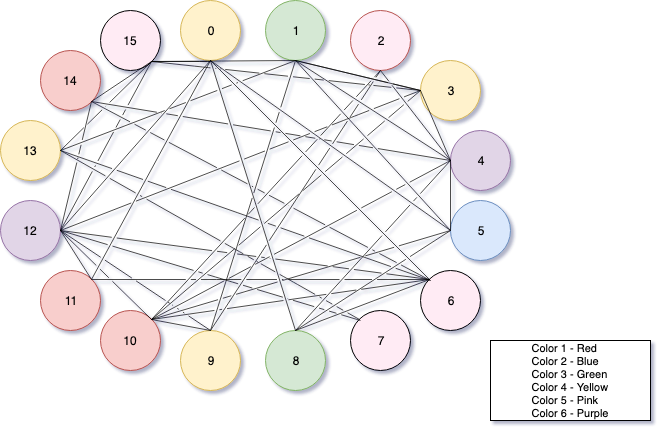
\includegraphics[width=10.0cm]{grap.png}
	\caption{Conflict Graph generated from the pseudo-random test-pattern set}
\end{figure}
\subsection*{(b)}

\end{document}
